\newpage
\section{Software engineering}
\label{sec:sw}

Within the previous section, different aspects of the project have been described both in electronic and mechanical terms. However, it is important to recall that the overall work is built in a quite complex system that incorporates together multiple actors. In fact, while we have been describing in detail for the past sections the development of one actor (a connected plush toy), the overall system is composed of different ones. Those actors are considered heterogeneous in both form and functionality. However, in order to have a working prototype, every single piece of the puzzle needs to perfectly fit within the big picture. Generally speaking, in the coming sections, we will indicate as the \textit{Toygether system} the set of different actors interacting together. Such system is illustrated in figure \ref{fig:SE_network_diagram} by a simplified diagram which aims to deliver an intuition of the different actors interacting together, without any networking details.

\begin{figure}[ht]
    \centering
    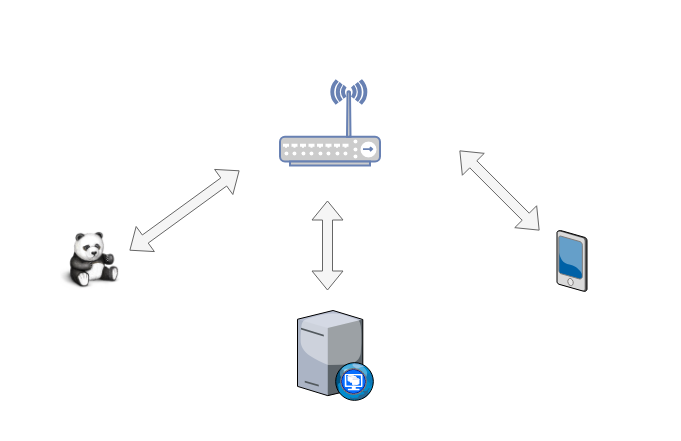
\includegraphics[scale=0.5]{images/SE_network_diagram.png}
    \caption{Simplified diagram of the overall system}
    \label{fig:SE_network_diagram}
\end{figure}

The previous figure introduces the three main categories of actors in the system: the \textbf{sever}, the \textbf{plush toy} and the \textbf{android user}. As previously mentioned, the illustration above corresponds to a simplification of the actual system by drawing a single representative for each class. However, it is crucial to understand that in a "real" context (outside of the purely prototyping domain) multiple clients and servers (in a distributed design) could operate in parallel. In the upcoming sections, in which design developments for each element will be discussed in detail, this vast reality needs to be considered to avoid architectures that fail to scale.

\medskip
In the following sections, we will first introduce the "common language" each actor will be required to speak in the system (subsection \ref{subsec:communication}). After the communication protocol has been defined, the server will be illustrated in detail (subsection \ref{subsec:server}); before eventually discuss the other client-class in the system defined as the Android app for parents (subsection \ref{subsec:android}).